\chapter{Modelli nella ricerca operativa}
\section{Problemi di ottimizzazione}
\subsection{Definizione funzione obiettivo e della formulazione del problema di ottimizzazione}
Data una funzione:
$$
    f:\mathbb{R}^n \to \mathbb{R} \longrightarrow \text{\textbf{Definita come \uline{funzione obiettivo}}}
$$

Un \textbf{problema di ottimizzazione} è formulabile come segue:
$$
    \begin{aligned}
        & \text{opt} & & f(x)  \\
        & \text{s.a.} & & x \in X \quad X \subseteq \mathbb{R}^n
    \end{aligned}
$$

$\mathbf{opt}$ è un \uline{operatore nella formulazione matematica generale} di un problema di ottimizzazione, viene usato per indicare l'operazione che si intende effettuare sulla funzione obiettivo, $opt \in \{min,max\}$

\subsection{Regione ammissibile}
X è detta regione ammissibile, cioè l'insieme delle soluzioni $x$ ammissibili dal problema.

\begin{minipage}[c]{0.45\textwidth}
    \vspace{0pt}
    \begin{itemize}
        \item Se $\mathbf{opt=min}$ abbiamo un \uline{problema di minimizzazione}
        \item Se $\mathbf{opt=max}$ abbiamo un \uline{problema di massimizzazione}
    \end{itemize}
\end{minipage}
\hfill
\begin{minipage}[c]{0.45\textwidth}
    \vspace{0pt}
    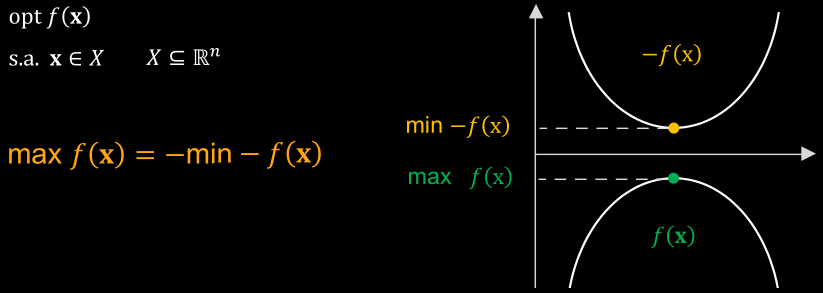
\includegraphics[width=\textwidth]{Immagini/minimizzazione-massimizzazione.png}
\end{minipage}

Le variabili che indicano i vincoli ai quali è soggetto il problema sono dette \textbf{variabili decisionali} e indentificano una soluzione del problema

\begin{minipage}[t]{0.45\textwidth}
    \subsubsection{Problema di massimizzazione}
    $$
    \begin{aligned}
        & \max f(x) & \longrightarrow \ & opt = \max \\
        & s.a. \ x \in X & \longrightarrow \ & \parbox[t]{5cm}{ \textbf{Variabili numeriche} in cui i valori identificano una soluzione del problema} \\
        & X \subseteq \mathbb{R}^n & \longrightarrow & \parbox[t]{5cm}{\textbf{Regione ammissibile}, ossia l'insieme delle soluzioni $x$ ammesse}
    \end{aligned}
    $$
\end{minipage}
\hfill
\begin{minipage}[t]{0.45\textwidth}
    \subsubsection{Problema di minimizzazione}
    $$
    \begin{aligned}
        & \min f(x) & \longrightarrow \ & opt = \max \\
        & s.a. \ x \in X & \longrightarrow \ & \parbox[t]{5cm}{ \textbf{Variabili numeriche} in cui i valori identificano una soluzione del problema} \\
        & X \subseteq \mathbb{R}^n & \longrightarrow & \parbox[t]{5cm}{\textbf{Regione ammissibile}, ossia l'insieme delle soluzioni $x$ ammesse}
    \end{aligned}
    $$
\end{minipage}

\subsection{In cosa consiste un problema di ottimizzazione?}
Un problema di ottimizzazione consiste nel determinare, se esistono, uno o più punti di $\min/\max\ \mathbf{x^*}$, assegnazioni di valori alle variabili decisionali $x$, della funzione obiettivo $f$ tra i punti $x \in X$

\newpage
\section{Tipologie di Ottimizzazione}
Quando parliamo di ottimizzazione di una funzione obiettivo possiamo avere diversi tipi di ottimizzazione

\subsection{Ottimizzazione NON vincolata}
La ricerca del/i punto/i di ottimo della funzione obiettivo viene condatta su tutto lo spazio di definizione della/e variabile/i di decisione

\begin{center}
    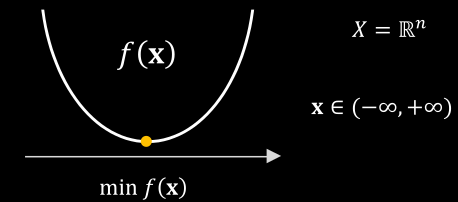
\includegraphics[scale=0.5]{Immagini/ott. non vincolata.png}
\end{center}


\subsection{Ottimizzazione vincolata}
La ricerca del/i punto di ottima della funzione obiettivo viene condotta su un sottoinsieme proprio dello spazio di definizione della/e variabile/i di decisione

\begin{center}
    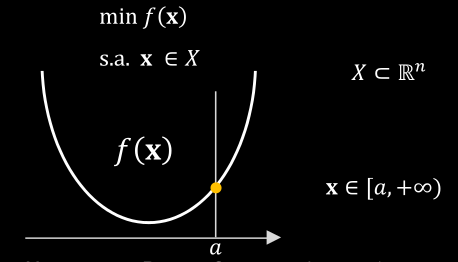
\includegraphics[scale=0.5]{Immagini/ott. vincolata.png}
\end{center}

\subsection{Ottimizzazione intera}
Le variabili assumono solo valori interi


{   \large
    $$
        \begin{aligned}
            opt f(x) \\
            s.a x \in X \\
            X \in \mathbb{Z}^n
        \end{aligned}
    $$
}

\subsection{Ottimizzazione binaria}
Le variabili assumono solo valore 0 o 1
{
    \large
    $$
        x \in \{0,1\}^n
    $$
}
\subsection{Ottimizzazione mista}
Alcune variabili assumono valori interni mentre altre variabili assumono solo valori binari.

Se non specifato altrimenti, si intende $X \subseteq \mathbb{R}^n$

\section{Programmazione Matematica}
\subsection{Definizione}
Quando l'insieme $X$ delle soluzioni ammissibili di un problema di ottimizzazione \uline{viene espresso attraverso un sistema di equazioni e disequazioni}, esso prende il nome di problema di \textbf{Programmazione Matematica}.

\subsection{Vincoli}
Un vincolo è un espressione del tipo


\begin{minipage}[c]{0.4\textwidth}
    {
    \large
    $$
        g_i(\mathbf{x})
        \left\{
        \begin{matrix}
        \geq \\
        = \\
        \leq
        \end{matrix}
        \right\}
        0
    $$
}
\end{minipage}
\hfil
\begin{minipage}[c]{0.4\textwidth}
    Dove intendiamo che $g_i(x)$ possa essere:
    \begin{itemize}
        \item $g_i(x) \geq 0$
        \item $g_i(x) = 0$
        \item $g_i \leq 0$
    \end{itemize}
\end{minipage}

Con $g_i:X \to \mathbb{R}$ funzione generica che lega tra loro le variabili decisionali.

In generale possiamo avere uno o più vincoli

\subsection{Definizione di Regione ammissibile (PM)}
La regione ammissibile è definita dall'insieme dei vincoli del problema

{
    \large
    $$
        X = \{x \in \mathbb{R}^n \text{ con } g_i(\mathbf{x})
        \left\{
        \begin{matrix}
        \geq \\
        = \\
        \leq
        \end{matrix}
        \right\}
        \ i=1,\dots,m
        \}   
    $$
}

Osserivamo, quindi, che abbiamo $m$ vincoli ed $n$ variabili
\begin{itemize}
    \item Se $\mathbf{x \in X}$ allora $x$ è \textbf{soluzione ammissibile}
    \item Se $\mathbf{x \not \in X}$ allora $x$ \textbf{non è una soluzione ammissibile}
\end{itemize}

\subsection{Tipologie di Regioni Ammissibili}

\subsubsection{Problema non ammissibile}
{
    \large

    $$
        X = \emptyset
    $$
}
Regione ammissibile vuota, nessuna soluzione ammissibile, problema mal posto

\subsubsection{Problema illimitato}
\begin{gather*}
    \forall c \in \mathbb{R},\ \exists x_C \in X : f(x_C) \leq c \quad \text{se } opt = min \quad \text{illimitato inferiormente} \\
    \forall c \in \mathbb{R},\ \exists x_C \in X : f(x_C) \geq c \quad \text{se } opt = min \quad \text{illimitato superiormente}
\end{gather*}

\subsubsection{Problema con soluzione ottima unica}

\subsubsection{Problema con più di una soluzione ottima (anche infinite)}
Tutte le soluzioni ottime hanno egual valore della funzione obiettivo

\newpage
\section{Ottimi globali e locali}

\subsection{Definizione Ottimo Globale}
La risoluzione di un problema di Programmazione Matematica consiste nel trovare una soluzione ammissibile che sia un \textbf{ottimo globale}, vale a dire un vettore $x^* \in X$ tale che :

\begin{gather*}
    f(x^*) \leq f(x) \quad \forall x \in X \quad \text{se } opt = min \\
    f(x^*) \geq f(x) \quad \forall x \in X \quad \text{se } opt = max
\end{gather*}

Un problema di ottimizzazione può avere:
\begin{itemize}
    \item Più di un ottimo locale
    \item Più di un ottimo globale
    \begin{itemize}
        \item Un punto di ottimo globale è anche di ottimo locale
    \end{itemize}
\end{itemize}

\subsection{Casi possibili}

\subsubsection{Programmazione Lineare}
In questo caso ci troviamo davanti ad un problema con questa formulazione:

$$
    opt f(x) = c^T x (lineare)
$$

la regione ammissibile è quindi formulabile in questo modo:

$$
        X = \{x \in \mathbb{R}^n \ :\  g_i(x)
        \left\{
        \begin{matrix}
        \geq \\
        = \\
        \leq
        \end{matrix}
        \right\}
        \ i=1,\dots,m
        \}
$$

con $g_i(x)=a^T_j x - b_i$ vincoli \textbf{lineari}

\subsubsection{Programmazione Lineare Intera}
In questo caso ci troviamo davanti ad un problema con questa formulazione

$$
    opt f(x) = c^T x (lineare)
$$

La regione ammissibile è quindi formulabile in questo modo

$$
        X = \{x \in \mathbb{Z}^n \ :\  g_i(x)
        \left\{
        \begin{matrix}
        \geq \\
        = \\
        \leq
        \end{matrix}
        \right\}
        \ i=1,\dots,m
        \}
$$

con $g_i(x)=a_j^T x - b_i$ vincoli \textbf{lineari} 

\subsubsection{Programmazione non lineare}
In questo caso ci troviamo davanti ad un problema con questa formulazione

$$
    opt f(x) \text{(lineare o non lineare)}
$$

La regione ammissibile è quindi formulabile in questo modo

$$
        X = \{x \in \mathbb{R}^n \ :\  g_i(x)
        \left\{
        \begin{matrix}
        \geq \\
        = \\
        \leq
        \end{matrix}
        \right\}
        \ i=1,\dots,m
        \}
$$

con $g_i(x)$ vincoli lineari o non lineari.

È importante notare come, in questo caso, almeno un vincolo o la funzione obiettivo sono non lineari